This chapter discusses the various methods used for testing and evaluating the system. This was done in three stages, starting with internal testing, continuing with a series of experiments performed on the system, and finalising with a user evaluation questionnaire taken by both students and researchers in different fields of biology. To note is that, due to the stochastic nature of the simulation, testing the system becomes difficult. Even identical initial conditions will result in visibly different outcomes after a matter of seconds. This can be seen in Figure~\ref{fig:randomoutcome}. Due to this, testing on a microscopic scale becomes impossible. The testing has to be carried out on a macroscopic level, while ensuing that the same patterns emerge from similar initial conditions.

\begin{figure}[!th]
	\centering
	\begin{minipage}[b]{0.49\textwidth}
		
\includegraphics[scale=0.37]{images/test1}
	\end{minipage}
	\hfill
	\begin{minipage}[b]{0.5\textwidth}
		
\includegraphics[scale=0.37]{images/test2}
	\end{minipage}
	\caption{\label{fig:randomoutcome}Different outcomes from same initial conditions; 20 second run}
\end{figure}

\section{Application Testing}
As Unity is primarily a game engine, part of the testing performed was visual testing. This involved running the simulation and observing any potential bugs. Due to the Agile development process, exploratory testing was also employed. With a rapidly evolving system, concrete tests would have proved obsolete after a few iterations. Using exploratory testing, new tests are being devised based on the results of the previous.

The unchanging part of the evolution, that is the algorithms handling the DNA sting required more robust testing in order to ensure functionality. These algorithms have undergone unit testing until deemed satisfactory.

\section{Experiments} \label{experiments}

A more high-level examination of the system dealt with the observation of the population under experimental conditions. Repeating the experiment multiple times while detecting the emergence of comparable patterns assured the functionality of the system.

The first step of the experiment was to run the simulation without interference. The expected result was an exponential growth in population until food became insufficient, followed by a small decline in the population number. The result was confirmed, as seen in Figure~\ref{fig:exp1}.

\begin{figure}[!th]
	\centering
	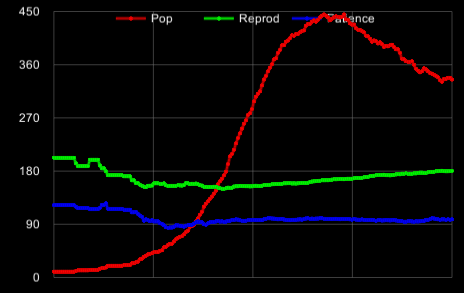
\includegraphics[scale=1.4]{images/exp1}
	\caption{\label{fig:exp1}Experiment 1: no interference}
\end{figure}

The next step of the experiment was to confirm the correlation between the availability of food and the population number. As expected, these are directly proportional; the more food available, the more will the population grow. Noteworthy is the tendency of blobs to become more ``selfish" as food grows scarcer. With a limited supply of food, the average reproduction threshold increases, causing blobs to require more sustenance until reproduction.

A similar observation can be made about the size of the food clusters. By altering the size of the clusters, the blobs' patience is affected. Larger clusters tend to evolve more patient populations, as food is more spread out, therefore increasing the merit of spending time in one particular area. Smaller clusters, however, have the opposite effect, as blobs find no reason to linger in an area after the food has been consumed.

The above two steps indicate a capability of blobs to adapt to their current environment.

The final part of the experiment deals with rapid changes in the environmental conditions with respect to the population. Firstly, a sudden influx in population is tested. This causes an even greater increase, as food is being consumed. However, due to unsustainable numbers, the population is rapidly reduced. Over a longer period of time, the population stabilises again. A graph detailing the artificial increase, natural increase, and sharp decrease can be seen in Figure~\ref{fig:exp4}

\begin{figure}[!th]
	\centering
	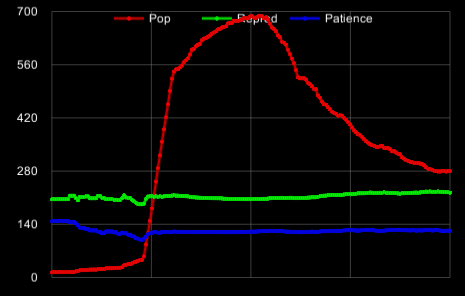
\includegraphics[scale=1.4]{images/exp4}
	\caption{\label{fig:exp4}Experiment 4: Artificial influx}
\end{figure}

Another method of influencing the environment is the creation of a hyper-dense food cluster. This would result in a localised population explosion, but a small spike in the overall population number. The only resulting observation was the slight decrease of both reproduction threshold and patience, as local changes can influence the global arithmetic mean.

\section{User Evaluation} \label{usereval}
As the project was reaching its final stages, a user evaluation was carried out. This involved the completion of a questionnaire by both fellow students and experts in the field of Biology. The feedback form in its entirety can be found in Appendix~\ref{appendix:b}. The purpose of the questionnaire was to measure the usability of the system, together with its capability of conveying useful information about the simulation. The design of the questionnaire was also important, lest the user be confused by any of the questions. A design similar to the System Usability Scale~\cite{lewis2009factor} was chosen for the 5-point scale questions regarding usability.

\subsection{A/B testing}

An approach similar to A/B testing, users were presented with three interface versions. Version 3, seen in Figure~\ref{fig:uiv3}, was presented as a control sample. Two other versions, presented in Figures~\ref{fig:uiv1}, and~\ref{fig:uiv2}, containing minor differences, were also presented. Unlike A/B testing, which requires a larger sample size, the results were not compared by the tester; users were asked to select their preferred interface out of the three. The choice was unanimous, all users having selected the control version as their favourite.

\begin{figure}[!th]
	\centering
	\begin{minipage}[b]{0.32\textwidth}
		\centering
		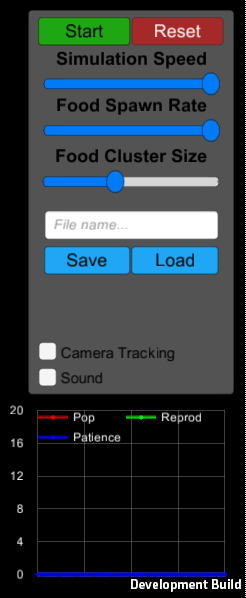
\includegraphics[scale=0.65]{images/uiv3}
		\caption{\label{fig:uiv3}Version 3, the control version of the interface}
	\end{minipage}
	\hfill
	\begin{minipage}[b]{0.32\textwidth}
		\centering
		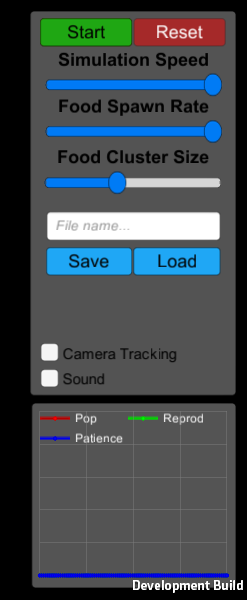
\includegraphics[scale=0.65]{images/uiv1}
		\caption{\label{fig:uiv1}Version 1, default interface}
	\end{minipage}
	\hfill
	\begin{minipage}[b]{0.23\textwidth}
		\centering
		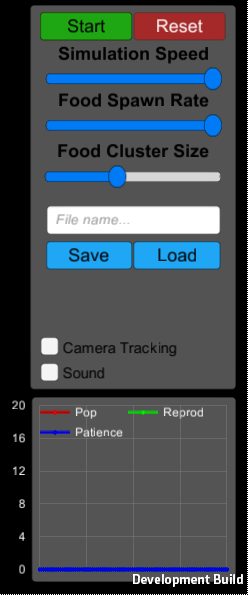
\includegraphics[scale=0.65]{images/uiv2}
		\caption{\label{fig:uiv2}Version 2, added labels on graph}
	\end{minipage}
\end{figure}

\subsection{Feedback Forms}
The users were asked to perform the same experimental steps as presented above, in order to enhance their understanding of the simulation. By noting their own observations of the occurrences, the user could test both the functionality and the usability of the system. The user responses to the long answer questions dealing with the observations were in line with the results received from the testing phase.

When asked about the usability of the system, the user responses were mostly positive, as seen in Figure~\ref{fig:genfeed}.
\begin{figure}[!th]
	\centering
	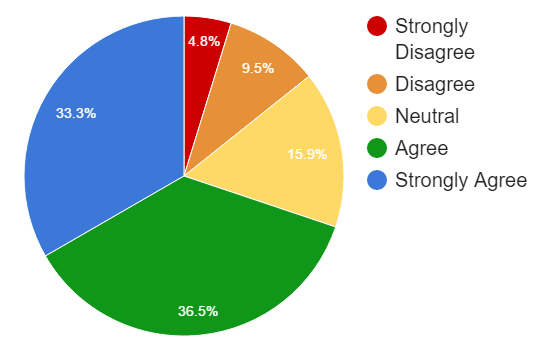
\includegraphics[scale=0.8]{images/genfeed}
	\caption{\label{fig:genfeed}An overview of the feedback received}
\end{figure}

While the interface was labelled as intuitive, some user were displeased with its visual appearance. Figures~\ref{fig:uifeed1} and~\ref{fig:uifeed2} present user responses for the interface-related questions.

\begin{figure}[!th]
	\centering
	\begin{minipage}[b]{0.49\textwidth}
		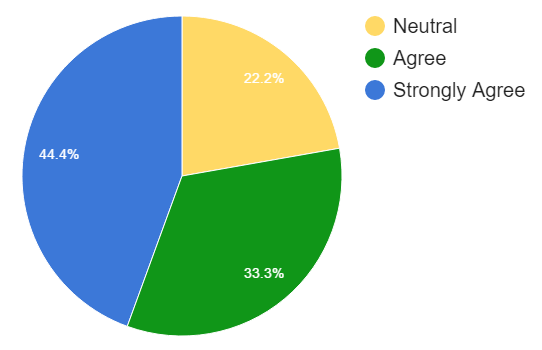
\includegraphics[scale=0.6]{images/q1}
		\caption{\label{fig:uifeed1}Q1: The interface is intuitive}
	\end{minipage}
	\hfill
	\begin{minipage}[b]{0.5\textwidth}
		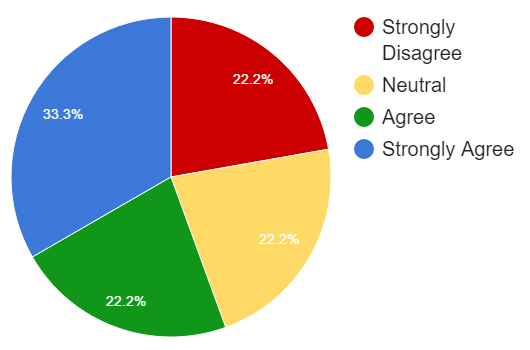
\includegraphics[scale=0.6]{images/q2}
		\caption{\label{fig:uifeed2}Q6: The interface is aesthetically pleasing}
	\end{minipage}
\end{figure}

Most users were in agreement that the simulation is explicit enough to draw conclusions from, however, it was also felt that more information should be provided. The manner in which information was provided was deemed satisfactory. The user responses for the simulation-related questions can be found in Figures~\ref{fig:simfeed1},~\ref{fig:simfeed2}, and~\ref{fig:simfeed3}.

\begin{figure}[h]
	\centering
	\begin{minipage}[b]{0.45\textwidth}
		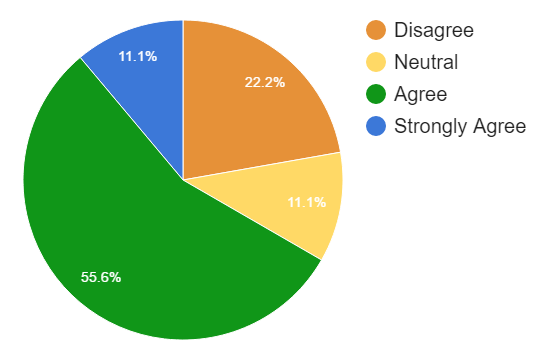
\includegraphics[scale=0.6]{images/q3}
		\caption{\label{fig:simfeed1}Q2: I am able to draw conclusions from the simulation}
	\end{minipage}
	\hfill
	\begin{minipage}[b]{0.45\textwidth}
		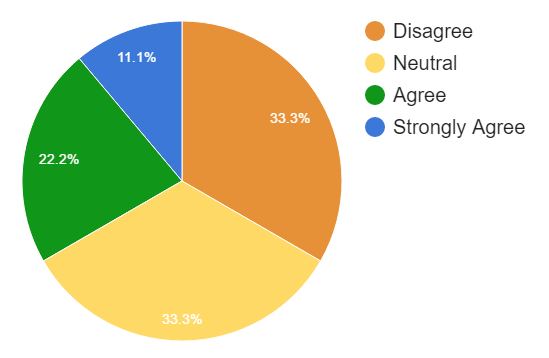
\includegraphics[scale=0.6]{images/q4}
		\caption{\label{fig:simfeed2}Q4: I am given enough information through the interface}
	\end{minipage}
	\newline
	\begin{minipage}[b]{0.45\textwidth}
		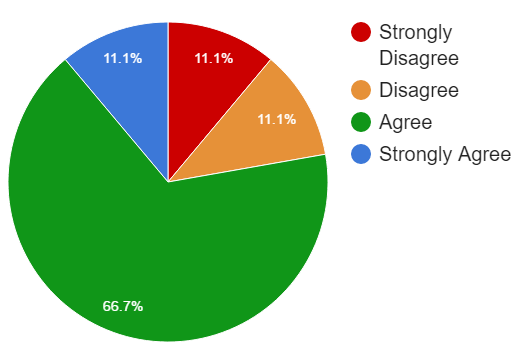
\includegraphics[scale=0.6]{images/q5}
		\caption{\label{fig:simfeed3}Q7: Information is conveyed effectively}
	\end{minipage}
\end{figure}

Feedback received on the questions concerning the software itself was positive, most users finding the controls easy to understand and use, and the system responsive. The answers can be found in Figures~\ref{fig:feed1} and~\ref{fig:feed2}.

\begin{figure}[!th]
	\centering
	\begin{minipage}[b]{0.49\textwidth}
		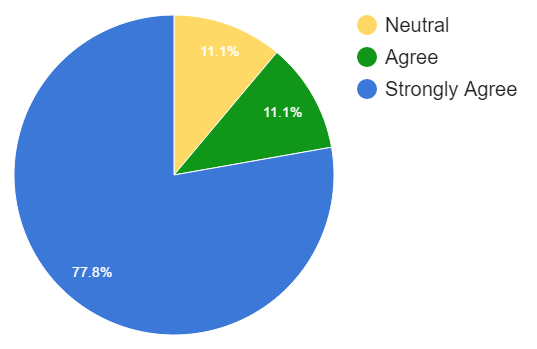
\includegraphics[scale=0.6]{images/q6}
		\caption{\label{fig:feed1}Q3: The controls are easy to use}
	\end{minipage}
	\hfill
	\begin{minipage}[b]{0.5\textwidth}
		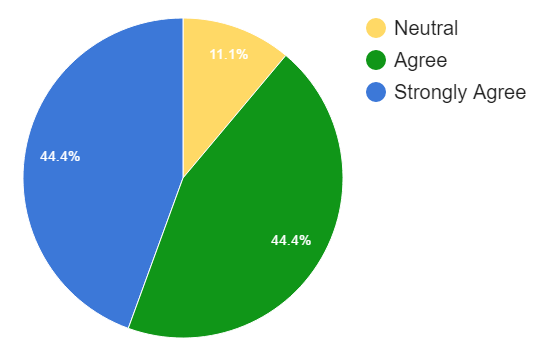
\includegraphics[scale=0.6]{images/q7}
		\caption{\label{fig:feed2}Q5: The software is responsive}
	\end{minipage}
\end{figure}

\subsection{Expert Opinion}

Throughout its evolution, the project was reviewed by Dr Simon Hickinbotham, who provided vital feedback for the project's development. His recommendations helped develop the biological side of the system.  A crucial suggestion with respect to aligning the simulation to real-life bacteria was the implementation of L\'evy walks as the blobs' primary movement pattern.

\section{Summary}
This chapter presented the evaluation process for the system from internal testing, to external user testing through a feedback questionnaire. The next chapter provides a summary of the project, as well as discuss project management issues and potential for further development.